\begin{table}[h!]

\section{Anhang und AN1E}

	\subsection{Für Prüfung}
	\begin{itemize}
	\item Definitionsbereich aufschreiben wenn Variable gebraucht wird.
	\item Induktion: \textbf{IA}: Induktionsannahme und \textbf{IE}: Induktionsschritt
	\end{itemize}
	
\begin{center}

% % % % % % % % % % % % % %
%Spezielle Ungleichungen
% % % % % % % % % % % % % %
	\begin{tabularx}{540pt}{|p{130pt}|X|}
		\hline
		\rowcolor{Gray}
		\multicolumn{2}{|c|}{\textbf{Spezielle Ungleichungen}}\\
		\hline
		Bernoulli-Ungleichung & 
		$(1 + a)^n > 1 + n \cdot a$ für $n \in N, n \geq 2, a \in R, a > -1, a\neq 0$\\
		\hline
		Binomische Ungleichung &
		$|a\cdot b|\leq\frac{1}{2}(a^2 + b^2)$\\
		\hline
		Dreiecksumgleichung & 	
		$\left|a+b\right|\leq\left|a\right|+\left|b\right|$\newline 						$\left|a-b\right|\leq\left|a\right|+\left|b\right|$ \newline
		$\left|a-b\right|\geq\left|\left|a\right|-\left|b\right|\right|$\\
		\hline
		Geometrisches Mittel & 
		$a_i\geq 0,\;n \in \mathbb{N},\;i \in \left\{1,2,...,n \right\}:$\\
		\hline
		Arithmetisches Mittel &
		$\sqrt[n]{a_1 a_2 \ldots a_n}\leq \frac{1}{n} \cdot \sum\limits _{i=1}^n a_i = 	\frac{a_1+a_2+...+a_n}{n}$\\
		\hline
		Natürliche Funktionen &
		$1+x\leq e^x\leq\frac{1}{1-x}$\newline
		$1-\frac{1}{x}\leq ln(x) \leq x-1$\\
		\hline
		Fakultät&
		$n! > 2^{n-1}$\\
		\hline
% % % % % % % % % % % % % % % % % %
%Summenzeichen und Binomischer Satz
% % % % % % % % % % % % % % % % % %
		\end{tabularx}
		\begin{tabularx}{540pt}{|X|X|X|X|}
		
		\hline
		\rowcolor{Gray}		
		\multicolumn{4}{|c|}{\textbf{Summenzeichen und Binomischer Satz}}\\
		\hline
		$\sum\limits _{i=1}^n a_i = \sum\limits _{i=1-j}^{n-j} a_{i+j}$& 
		$\left(a+b\right)^n = \sum\limits _{i=0}^n \left(\stackrel{n}{i}\right)a^{n-i}\cdot b^i$&
		$\left(\stackrel{n}{i-1}\right)+\left(\stackrel{n}{i}\right)=\left(\stackrel{n+1}{i}\right)$&
		$\left(\stackrel{n}{i}\right)=\frac{n\left(n-1\right)\cdot...\cdot\left(n-i+1\right)}{1\cdot 2\cdot 3\cdot...\cdot i}$\\
		\hline
		$\left(\stackrel{n}{i}\right)=\frac{n!}{i!\left(n-i\right)!}$&
		$\left(\stackrel{n}{i}\right)=\left(\stackrel{n}{n-i}\right)$&
		$\left(\stackrel{n}{0}\right)=1$&
		$\left(\stackrel{0}{0}\right)=1$\\
		\hline
		\multicolumn{2}{|l|}{$(2n+2)!=(2n+2)(2n+1)((2n)!)$}&
		&
		\\
		
		\end{tabularx}
% % % % % % % % % % % % % % % % % %
%Transformationen
% % % % % % % % % % % % % % % % % %
		\begin{tabularx}{540pt}{|p{150pt}|X|}
		\hline
		\rowcolor{Gray}
		\multicolumn{2}{|c|}{\textbf{Transformationen}}\\
		\hline
		
		$\mathbf{\pm \; {\color{red}a} \cdot f( \; \pm \; {\color{blue}b} \cdot ( \; x \; \pm \; 
						{ \; \color{green}c})) \; \pm \; {\color{cyan}d}}$ &
							1. \textbf{{\color{red}a}} Vertikale Streckung um \textbf{a} bzw. Spiegelung an x bei \textbf{-a}\newline
							2. \textbf{{\color{blue}b}} Horizontale Streckung um \textbf{1/b} bzw. Spiegelung an y bei \textbf{-b}\newline					
							3. \textbf{{\color{green}c}} Verschiebung nach links (\textbf{+c}) oder rechts (\textbf{-c})\newline
							4. \textbf{{\color{cyan}d}} Verschiebung nach oben (\textbf{+d}) oder unten (\textbf{-d})\\	
		\hline
		\end{tabularx}
		
% % % % % % % % % % % % % % % % % %
%Transformationen
% % % % % % % % % % % % % % % % % %
		\begin{tabularx}{540pt}{|p{270pt}|X|}
		\hline
		\rowcolor{Gray}
		\multicolumn{2}{|c|}{\textbf{Gerade/Ungerade Funktionen}}\\
		\hline
		Gerade Funktionen(Achsensymmetrisch):\newline \textbf{$f(-x) = f(x)$} &
		
		Ungerade Funktionen(Punktsymmetrisch):\newline \textbf{$f(-x) = -f(x)$}\\
		\hline
		\end{tabularx}
		
		\end{center}
		\end{table}
	
% % % % % % % % % % % % % % % % % %
%uneigentliche Grenzwerte
% % % % % % % % % % % % % % % % % %	
		\begin{table}[h!]
		\begin{center}
		\begin{tabularx}{540pt}{|X|X|X|X|X|}
		\hline
		\rowcolor{Gray}		
		\multicolumn{5	}{|c|}{\textbf{uneigentliche Grenzwerte}}\\
		\hline
		\textbf{Bestimmte Form}&
		$\infty+\infty = \infty$& 
		$-\infty - \infty = -\infty$&
		$\infty \cdot \infty = \infty$&
		$-\infty \cdot(\infty) = -\infty$\\	
		&
		$\dfrac{1}{\infty}$ = 0&
		$\dfrac{\infty}{0+} = \infty$&
		$\dfrac{\infty}{0-} = -\infty$&
		\\										
		\hline
		\textbf{Unbestimmte Form}&
		$\dfrac{0}{0}$&
		$\dfrac{\infty}{\infty}$&
		$\infty - \infty$&
		$0^0$\\
		&
		$\infty^0$&
		$1^\infty$&
		&
		\\
		\hline	
		\end{tabularx}
% % % % % % % % % % % % % % % % % %
%Trigonometrische Funktionen
% % % % % % % % % % % % % % % % % %			
		\begin{tabularx}{540pt}{|p{170pt}|X|}
		\hline
		\rowcolor{Gray}
		\multicolumn{2}{|c|}{\textbf{Trigonometrische Funktionen}}\\
		\hline
		
		
		\begin{tabular}{c|c|c|c|c}

		Winkel & Bogen & sin & cos & tan\\
		\hline
		$0^\circ$  & 0 & 0& 1&0\\
		\hline
		$30^\circ$  &$\dfrac{\pi}{6}$ & $\dfrac{1}{2}$ &$\dfrac{\sqrt{3}}{2}$ &$\dfrac{\sqrt{3} }{ 3}$\\
		\hline
		$45^\circ$ & $\dfrac{\pi}{4}$ &$\dfrac{\sqrt{2}}{2}$ &$\dfrac{\sqrt{2}}{2}$ & 1\\
		\hline
		$60^\circ$ & $\dfrac{\pi}{3}$&$\dfrac{\sqrt{3}}{2}$ & $\dfrac{1}{2}$&$\sqrt{3}$\\
		\hline
		$90^\circ$ &$\dfrac{\pi}{2}$ & 1  & 0 & $\pm \infty$\\		

		\end{tabular}
		&
	
		\begin{tabular}{|c|c|c|c|}
		\hline
		$\alpha$               &$\sin\alpha$ &$\cos\alpha$            &$\tan\alpha$  \\
    	$\sin\alpha$           &-            &$\sqrt{1-\cos^2\alpha} $&$\dfrac{\tan\alpha}{\sqrt{1+\tan^2\alpha}}$  \\
    	$\cos\alpha$           &$\sqrt{1-sin^2\alpha}$           &-                       &$\dfrac{1}{\sqrt{1+\tan^2\alpha}}$ \\
    	$\tan\alpha$           &$\dfrac{\sin\alpha}{\sqrt{1-sin^2\alpha}}$           &$\dfrac{\sqrt{1-cos^2\alpha}}{\cos\alpha}$                      &-  \\
		\hline
		\end{tabular}
		\\
		\hline	
		\end{tabularx}
		
	\begin{tabularx}{540pt}{|p{130pt}|p{150pt}|X|}
		$sin^2\alpha+cos^2\alpha = 1$ &
		$ \dfrac{\sin\alpha}{\cos\alpha} = \tan\alpha$ &
		$\sin(\alpha \pm \beta) = \sin\alpha cos\beta \pm \cos\alpha \sin\beta$ \\
		
		$\cos(2\alpha)= \cos^2\alpha-\sin^2\alpha$ &
		$\sin(2\alpha)= 2\sin\alpha\cos\alpha$&
		$\cos(\alpha \pm \beta)= \cos\alpha\cos\beta \mp \sin\alpha \sin\beta$\\
		
		$\sin\dfrac{\alpha}{2} = \sqrt{\dfrac{1}{2}(1-\cos\alpha)}$ &
		$\cos\dfrac{\alpha}{2} = \sqrt{\dfrac{1}{2}(1+\cos\alpha)}$&
		$\tan\dfrac{\alpha}{2} = \dfrac{\sin\alpha}{1+\cos\alpha} = \dfrac{1-\cos\alpha}{\sin\alpha}$\\

		$\sin^2\alpha = \dfrac{1}{2}(1-\cos 2\alpha)$&
		$\cos^2\alpha = \dfrac{1}{2}(1+\cos 2\alpha)$&
		Cosinussatz: $c^2=a^2+b^2-2ab\cdot \cos\gamma$\\
		
		\multicolumn{2}{|c|}{
		$\sin\alpha + \sin \beta = 2\sin\dfrac{\alpha + \beta}{2}\cos\dfrac{\alpha - \beta}{2}$}&
		
		$\tan\alpha \pm \tan\beta = \dfrac{\sin(\alpha\pm\beta)}{\cos\alpha\cos\beta}$\\
		
		\multicolumn{2}{|c|}{$cos\alpha + cos\beta = 2\cos\dfrac{\alpha + \beta}{2}\cos\dfrac{\alpha-\beta}{2}$}&
		$\cos\alpha\cos\beta = \dfrac{1}{2}[\cos(\alpha - \beta) + \cos(\alpha+\beta)]$\\
		
		\multicolumn{2}{|c|}{$\sin\alpha\cos\beta = \dfrac{1}{2}[\sin(\alpha - \beta) + \sin(\alpha+\beta)]$}&
		$\sin\alpha\sin\beta = \dfrac{1}{2}[\cos(\alpha - \beta) - \cos(\alpha+\beta)]$
		\\
		
		\multicolumn{2}{|c|}{
		Schnittwinkel zweier Geraden: $\tan\delta = \dfrac{m_1-m_2}{1+m_1 m_2}$}&
		Orthoganalitätsbedingung: $m_1\cdot m_2 = -1$\\
	\hline
		
		\end{tabularx}	
	
		
		
		
		


% % % % % % % % % % % % % % % % % %
%Hyperbolicus Funktionen
% % % % % % % % % % % % % % % % % %			
		\begin{tabularx}{540pt}{|X|X|X|}
	\hline		
	\rowcolor{Gray}
	\multicolumn{3}{|c|}{\textbf{Hyperbolicus Funktionen}}\\
	\hline
		$\sinh x = \frac{1}{2}(e^x-e^{-x})$&
		$\cosh x = \frac{1}{2}(e^x+e^{-x})$&
		$\tanh x = \dfrac{\sinh x}{\cosh x}$\\
		
	\hline
		$arsinh(x) = \ln(x+\sqrt{x^2+1})$&
		$arcosh(x) = \ln(x+\sqrt{x^2-1})$ \newline mit $x\in[1,\infty)$ &
		$artanh(x)=\frac{1}{2}\ln\dfrac{1+x}{1-x}$ \newline mit $x\in \mathbb R \backslash[-1,1]$\\
	\hline
	 $\cosh^2 x - \sinh^2 x = 1$&
	$ e^x = \cosh x + \sinh x$&
	\\
	 \hline
		\end{tabularx}
		\end{center}
		\end{table}


% % % % % % % % % % % % % % % % % %
%Partialbruchzerlegung
% % % % % % % % % % % % % % % % % %	
		\begin{table}[h!]
		\begin{center}
		\begin{tabularx}{540pt}{|p{210pt}|X|}
		\hline
		\rowcolor{Gray}
		\multicolumn{2}{|c|}{\textbf{Partialbruchzerlegung}}\\
		\hline
		
		1. Nenner hat n verschiedene Nullstellen&
		$q(x) = k(x-x_1)(x-x_2)...(x-x_n)$\\
		
		&
		Ansatz: $\dfrac{p(x)}{q(x)}=\dfrac{A_1}{x-x_1}+\dfrac{A_2}{x-x_2}+...+\dfrac{A_n}{x-x_n}$\\
		\hline
		
		2. Nenner hat n reelle Nullstellen \newline(mehrfache Nullstellen)&
		$q(x) = k(x-x_1)^{n_1}(x-x_2)^{n_2}...(x-x_n)^{n_i}$\\
		&
		Ansatz: $\dfrac{p(x)}{q(x)}=\dfrac{A_1}{(x-x_i)}+\dfrac{A_2}{(x-x_i)^2}+...+\dfrac{A_{n_i}}{(x-x_i)^{n_i}}$\\
		\hline
		
		3. Nenner enthält nicht zerlegbare Nullstellen&
		$x^2+bx+c$\\
		
		&
		Ansatz: $\dfrac{Bx+C}{x^2+bx+c}$\\
		\hline
		\end{tabularx}
% % % % % % % % % % % % % % % % % %
%Kurvendiskussion
% % % % % % % % % % % % % % % % % %	
		
		\begin{tabularx}{540pt}{|p{30pt}|X|}
		\hline
		\rowcolor{Gray}
		\multicolumn{2}{|c|}{\textbf{Kurvendiskussion Programm}}\\
		\hline
		
		1& \textbf{Definitionsmenge/Wertemenge}\\
		\hline
		2& \textbf{Symmetrien} (gerade$\leftrightarrow$ Achsensymmetrie, ungerade $\leftrightarrow$Punktsymmetrie), \textbf{Periodizität} ($k\pi$),\newline 
		\textbf{Transformation} $(a\cdot f(bx+c)+d)$\\
		\hline
		3&\textbf{Nullstellen} ($f(x) = 0$)\\
		\hline
		4&\textbf{Stetigkeit}(voraussetzung für Differenzierbarkeit), \textbf{Differenzierbarkeit} ($f', f'', f'''$)\newline
		Hinweis: Zu beachten sind hier besonders Lücken, Polstellen, Sprungstellen, Oszillationsstellen\\
		\hline
		5& A) \textbf{Monotonieverhalten}, \textbf{Extremalstellen}\newline
		   B) \textbf{Krümmungsverhalten, Wendestellen/Wendetangenten}\\
		\hline
		6& \textbf{Grenzverhalten} $x\rightarrow \pm\infty$/\textbf{Randstellen/Polstellen}\\
		\hline		
	
		
		\end{tabularx}
		
% % % % % % % % % % % % % % % % % %
%Spezielle Grenzwerte
% % % % % % % % % % % % % % % % % %	
		
		\begin{tabularx}{540pt}{|p{150pt}|p{210pt}|X|}
		\hline
		\rowcolor{Gray}
		\multicolumn{3}{|c|}{\textbf{Spezielle Grenzwerte}}\\
		\hline
		$ \lim\limits_{x \to 0} \dfrac{\sin{x}}{x} = 1 \Rightarrow \dfrac{\sin{4x}}{x} = 4$&
		$ \lim\limits_{x \to \infty} \dfrac{x^{\alpha}}{a^{\beta x}} = 0 \:(a>1;\:\alpha, \beta > 0 ) $&
		$ \lim\limits_{x \to \infty} \dfrac{(\ln x)^\alpha}{x^{\beta}} = 0 $\\
		
		$ \lim\limits_{x \to \infty} \left(1+\dfrac{a}{x}\right)^x=e^a $&
		$ \lim\limits_{x \to 0} (1+x)^{\dfrac{1}{x}}=e $&
		$ \lim\limits_{x \to 0} \dfrac{a^x-1}{x}=\ln a $\\

		$ \lim\limits_{x \to 0} \dfrac{\log_a(x+1)}{x} = \dfrac{1}{\ln a} $&
		$ \lim\limits_{x \to \infty} \dfrac{(\ln x)^\alpha}{x^{\beta}} = 0 $&
		$ \lim\limits_{x \to \infty} \dfrac{x}{\tan x} $\\

		$ \lim\limits_{x \to 1} \dfrac{\ln{x}}{x-1} = 1 $&
		$ \lim\limits_{x \to 0+} x \ln{x} = 0 $&
		$ \lim\limits_{x \to 0} \dfrac{e^x-1}{x}=1 $\\

		$ \lim\limits_{x \to 0} \dfrac{x}{1-e^{-x}}=1 $&
		$ \lim\limits_{x \to \infty} \sum\limits_{k=0}^n q^k = \begin{cases}+\infty &q \geq 1\\ \dfrac{1}{1-q} &|q|<1 \\ $unbest.divergent$ & q\leq -1\end{cases} $&
		$ \lim\limits_{\alpha \to 0} \dfrac{(1+x)^{\alpha}-1}{x} = \alpha $\\

		$ \lim\limits_{x \to \infty} \dfrac{x^n}{n!} = 0 \:(x>0) $&
		$ \lim\limits_{x \to \infty} \dfrac{x^k}{q^x}=0 \:(q>1; \:k\in \mathbb{N}) $&
		$ \lim\limits_{x \to \infty} \sqrt[x]{p}=1 $\\
		\hline
		\end{tabularx}
	
	\end{center}
	\end{table}	
	
	
% % % % % % % % % % % % % % % % % %
%Zahlenfolge
% % % % % % % % % % % % % % % % % %	
		\begin{table}[h!]
		\begin{center}
		
		\begin{tabularx}{540pt}{|p{270pt}|X|}
		\hline
		\rowcolor{Gray}
		\multicolumn{2}{|c|}{\textbf{Zahlenfolge}}\\
		\hline
		
		arithmetische Folge& geometrische Folge\\
		
		$a_1 = c $ und $a_n{n+1}=a_n+d$ \newline($d=a_{an+1}-a_n \Rightarrow$ Monotonie) &
		$a_1 = c $ und $a_{n+1}=q\cdot a_n$ \newline$\bigg(q=\dfrac{a_{n+1}}{a_n} \Rightarrow$ Monotonie$\bigg)$\\
		\hline
		
		\multicolumn{2}{|c|}{Grenzwerte von rekursiven Folgen}\\
		\hline
		1. \textbf{Monotonie} annehmen(ev. erste Glieder Berechnen)&
		$\Rightarrow$ mit vollständiger Induktion beweisen\newline
		Verankerung: $f_1 < f_2$\newline
		Vererbung  : $f_n < f_{n+1}$\\
		\hline
		2. \textbf{Hypothetischer Grenzwert ausrechnen} & 
		Beschränktheit annehmen und Limes ziehen\newline
		$f_n = f_{n+1}$ in unendlichkeit (für $f_n  $ und $ f_{n+1}$einfach $x$ einsetzen)\\
		\hline
		3. \textbf{Beweisen} & Beschränktheit mittels des hypotthetischen Grenzwertes und vollständiger Induktion beweisen\\
		\hline		
		\end{tabularx}
		
	
% % % % % % % % % % % % % % % % % %
%Asymptotenbestimmung
% % % % % % % % % % % % % % % % % %	
		\begin{tabularx}{540pt}{|p{50pt}|p{80pt}|X|X|}
		\hline
		\rowcolor{Gray}
		\multicolumn{4}{|c|}{\textbf{Asymptote}}\\
		\hline
		
		\multicolumn{4}{|c|}{Asymptote einer gebrochen rationalen Funktion
		 $r(x)=\dfrac{p_m(x)}{Q_n(x)}$}\\
		\hline
		
		&$m<n$ & $m=n$ & $m>n$\\
		\hline
		
		$\lim\limits_{x\rightarrow\pm\infty} = $&
		0&
		$\dfrac{a_m}{b_n}$&
		$\pm\infty$\\
		
		Asymptote&
		x-Achse&
		Parallel zur x-Achse: \newline
		$y=\dfrac{a_m}{b_n}$&
		Ganzrationaler Teil der Pol. division\\
		
		\hline
		\multicolumn{4}{|c|}{für Funktionen, die nicht gebrochenrational sind(existiert nur wenn alle Grenzwerte existieren)}\\
		\hline
		\multicolumn{4}{|c|}{Asymptote: $g=ax+b \Rightarrow \lim\limits_{x\to \infty}(f(x)-ax-b)=0$}\\
		
		
		\multicolumn{2}{|c}{$a= \lim\limits_{x\to\infty}\dfrac{f(x)}{x}$ oder $a= \lim\limits_{x\to\infty}f'(x)$}&
		\multicolumn{2}{|c|}{$b=\lim\limits_{x\to\infty}f(x)-ax$}\\
		\hline
		\end{tabularx}		

% % % % % % % % % % % % % % % % % %
%Differentialrechnung
% % % % % % % % % % % % % % % % % %	
		\begin{tabularx}{540pt}{|X|X|}
		\hline
		\rowcolor{Gray}
		\multicolumn{2}{|c|}{\textbf{Differentialrechnung}}\\
		\hline
		
		$f'(x_0) = \lim\limits_{h\to 0}\dfrac{f(x_0+h)-f(x_0)}{h}$&
		Tangentengleichung: $t(x)=f(x_0) + f'(x_0)(x-x_0)$\\
		\hline
		Normalengleichung: $n(x)=\dfrac{x_0-x}{f'(x_0)}+f(x_0)$&
		Mittelwertsatz:  $\dfrac{f(b)-f(a)}{b-a}=f'(\xi)$\\
		\hline
		abs. Fehler: $|\Delta y|\approx|dy|=|f'(x)|\cdot|\Delta\delta|$&
		rel. Fehler: $\bigg|\dfrac{f'(x)}{y}\bigg|\cdot |dx| \leq \bigg|\dfrac{f'(x)}{f(x)}\bigg|\cdot|\Delta\delta|$\\
		\hline
		
		$f'(x) \geq 0$ Monoton steigend $\uparrow$ &
		$f'(x) \leq 0$ Monoton fallend $\downarrow$\\
		\hline

		\end{tabularx}	
		

	\end{center}
	\end{table}	
	
		\begin{table}[h!]
		\begin{center}

		\begin{tabularx}{550pt}{|X|X|}
		
		\hline
		konvex(linkskrümmung) $ \Leftrightarrow f' \uparrow \Leftrightarrow f''\geq 0$&
		konkav(rechtskrümmung) $ \Leftrightarrow f' \downarrow \Leftrightarrow f''\leq 0$\\
		\hline
		\multicolumn{2}{|c|}{Extremalstelle: $f'(x_0) = 0$ /Wendepunkt: $f''(x_0) = 0$ potentieller Kandidat }\\
		\multicolumn{2}{|c|}{ $f''(x_{0}) = 0,{ }...{ }, f^{n-1}(x_{0}) = 0, f^{n}(x_{0}) \neq 0\left\{\begin{array}{l}
				\mbox{n gerade} \left\{
					\begin{array} {l} 
						f^{n}(x_{0}) > 0 \Rightarrow \mbox{relatives Minimum bei } x_0 \\ 
						f^{n}(x_{0}) < 0 \Rightarrow \mbox{relatives Maximum bei } x_0  
					\end{array} \right. \\
				\mbox{n ungerade} \Rightarrow \mbox{Wendestelle bei } x_0 (\mbox{Terrassenpunkt} f'(x_0)=0) 
			\end{array} 
			\right.
			$}\\
		\hline
		\end{tabularx}	

% % % % % % % % % % % % % % % % % %
%Bernoulli
% % % % % % % % % % % % % % % % % %	
		\begin{tabularx}{550pt}{|X|X|X|}
		\hline
		\rowcolor{Gray}
		\multicolumn{3}{|c|}{\textbf{Benoulli}}\\
		\hline
		
		\multicolumn{3}{|c|}{$\lim\limits_{x\downarrow x_0}\dfrac{f_1(x)}{f_2(x)}$=$\lim\limits_{x\downarrow x_0}\dfrac{f_1'(x)}{f_2'(x)}$ das gilt für $\dfrac{0}{0}$ oder den$\dfrac{\pm \infty}{\pm \infty}$ fall. }\\
		\hline
		
		$0\cdot \pm \infty \Rightarrow\dfrac{f_1}{\frac{1}{f_2}}=\dfrac{0}{0}$ oder
		$\dfrac{f_2}{\frac{1}{f_1}}=\dfrac{\pm \infty}{\pm \infty}$ &
		$\infty - \infty \Rightarrow \dfrac{\frac{1}{f_2}-\frac{1}{f_1}}{\frac{1}{f_1 \cdot f_2}} $ &
		bei $f^g = 1^\infty , 0^0, \infty^0 \Rightarrow e^{g\cdot \ln(f)}$\\
		\hline
		
		\end{tabularx}			

% % % % % % % % % % % % % % % % % %
%Taylor-Polynom
% % % % % % % % % % % % % % % % % %	
%tabularx: Damit inhalt der Tabelle zentriert ist
\renewcommand{\tabularxcolumn}[1]{>{\normalsize\centering\arraybackslash}m{#1}}
		\begin{tabularx}{550pt}{|X|}
		\hline
		\rowcolor{Gray}
		\textbf{Taylor-Polynom}\\
		\hline
		($x_0$=Entwicklungspunkt)$\quad f(x_0+h)=f(x_0) + f'(x_0)h + \frac{f''(x_0)}{2}h^2 + \frac{f'''(x_0)}{3!}h^3 + \ldots + \frac{f^{(n)}(x_0)}{n!}h^n + R_n(x_0, h)$\\
		\hline
		$R_n$(\textbf{Lagrange}):$\quad R_n(x_0, h) = \dfrac{f^{(n+1)}(x_0 + \theta h)}{(n+1)!}h^{n+1}, (0 < \theta < 1)$\\
		
		$\lim\limits_{n \to \infty} R_n(x_0, h) = 0 \Longrightarrow f(x_0+h) = \sum\limits_{n=0}^{\infty} \dfrac{f^{(n)}(x_0)}{n!}h^n$\\
		\hline			
		\textbf{MacLaurinsche-Form} (gilt für $ x_0=0, h=x ):  f(x)=\sum\limits_{k=0}^{n} \dfrac{f^{(k)}(0)}{k!} \cdot x^k + R_n $ \\
		$R_n = \dfrac{f^{(n+1)}(\theta x)}{(n+1)!} \cdot x^{n+1}, (0 < \theta < 1)$\\
		\hline
		
		\end{tabularx}
%aufhebender Befehl
\def\tabularxcolumn#1{p{#1}}



	\begin{tabularx}{550pt}{| X  X X|}
		\hline
		\rowcolor{Gray}
		\multicolumn{3}{c}{\textbf{Funktionsgraphen}}\\
		\hline
	e-Funktion & Logarithmusfunktion & $\frac{1}{x}- Funktion$\\
	
	\raisebox{-.7\totalheight}{\includegraphics[width = 3.5cm]{bilder/2_Efunktion.png}} & \raisebox{-.7\totalheight}{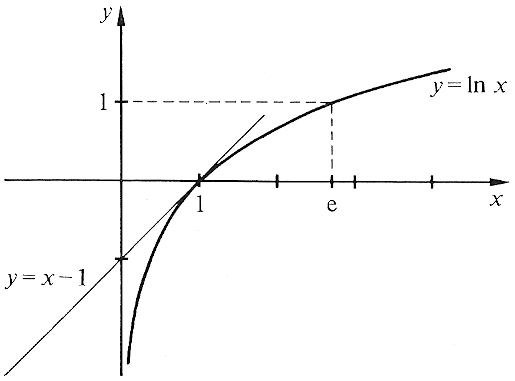
\includegraphics[width =  5cm]{bilder/2_lnFunktion.png}}&
	\raisebox{-.7\totalheight}{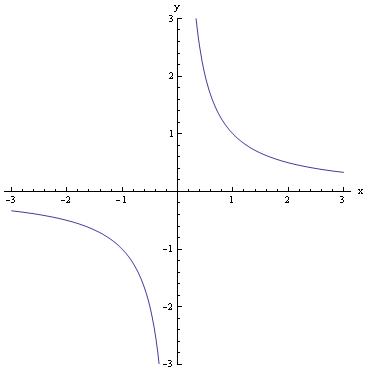
\includegraphics[width = 3.5cm]{bilder/2_1toxFunktion.png}} \\
	\hline
\end{tabularx}
		\end{center}
		\end{table}	
